\begin{opin}{\guscolor}{Gustavo}

\subsubsection{Introducción a la neurodidáctica}

Parece una evidencia científica que sin emoción no hay aprendizaje. Es necesario despertar en los adolescentes el interés por las matemáticas en particular y por el conocimiento en general. Y para ello podemos hacer uso de técnicas que permitan emocionar a los alumnos sobre lo que están haciendo y de esta manera conseguir que, seguramente de manera inconsciente para ellos, aprendan los contenidos básicos necesarios para su desarrollo personal.


Hay gente que equipara los términos neurodidáctica y neuroeducación, ambos asociados a la neurociencia. En nuestra clase lo vamos a diferenciar en función de:

\begin{itemize}
\item Neuroeducación: Manera en la que el cerebro aprende
\item Neurodidáctica: Manara en la que el docente lleva a la práctica la neuroeducación
\end{itemize}

\subsubsection{Neuroeducación por otra escuela}

Se puede acceder al video en el siguiente enlace:

\href{https://www.youtube.com/watch?v=QiRqCKUiRDc\&feature=youtu.be}{https://www.youtube.com/watch?v=QiRqCKUiRDc\&feature=youtu.be}
\paragraph{Partes del cerebro. Aprendizaje =  DIVERSION * K}
Las cosas que yo pienso \textmd{se ejecutan} mediante la parte del cerebro prefrontal, que sería la parte de la cabeza que usan los futbolistas para rematar un balón. Se denomina función ejecutiva y se encarga de:
\begin{itemize}
\item La concentración
\item El control de impulsos
\item La memoria a corto plazo
\end{itemize}
La amígdala es la parte del cerebro que se encarga de la emoción y es “la gasolina” de la función ejecutiva.


\begin{minipage}[hbtp]{1.0\linewidth}
\centering
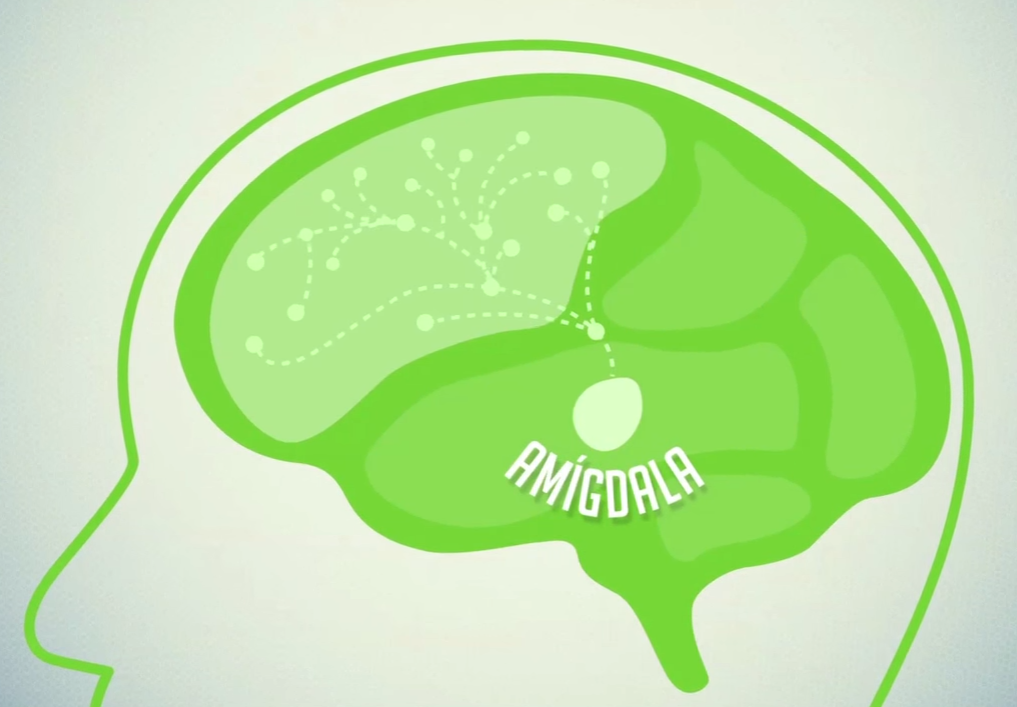
\includegraphics[scale=0.2]{img/cerebrogus.png}
\captionof{figure}{Esquema de la posición de la amígdala en el cerebro humano.}
\end{minipage}

Por simplificar mucho hasta el momento, la parte racional está en el prefrontal y la parte emocional está en la amígdala.


Con esto se explicaría que si estás emocionado con algo, tengas una mejor concentración y por tanto un mejor aprendizaje. En realidad, el cerebro tiene muchas partes y para que el proceso de aprendizaje sea total se deberían emplear todas las regiones y funciones del cerebro.


Como dijo \textbf{Helena Lopez Casares en la conferencia que dio el 20 de septiembre en el Campus Vicálvaro} sobre inteligencias múltiples, hay estudios que demuestran que personas con problemas en la parte del cerebro que controla las emociones son incapaces de tomar una decisión, con lo cual se demuestra la importancia de todas las partes del cerebro deben estar activas y conectadas.

\paragraph{Educación bulímica. Matemáticas, Historia y Filosofía}
Me ha gustado mucho la afirmación que hace Javier Blumenfeld: “Tenemos una especie de educación bulímica: yo te meto contenidos y tú me los vomitas en el examen”. Esto es lo que yo llamo metodología tradicional de la enseñanza.


En este caso sí haría diferenciación por asignaturas y lo aplicaría a mi experiencia personal. En el caso de las matemáticas, aparte de que siempre me han gustado más, he sido capaz de aprenderlas y es muy difícil que se me olviden. O si hay algo que no tengo claro, con un simple repaso sería capaz de recordarlo. Estas matemáticas las he aprendido bajo un contexto de educación bulímica y aun así he sido capaz de aprenderlas. Sin embargo, en asignaturas como historia, filosofía, u otras asignaturas que la manera de aprobar consistía en la memorizar y repetir lo memorizado en el examen, no he recordado nunca nada de adulto.


Sin embargo, es curioso como a día de hoy sí me siento atraído por la historia y por los pensamientos filosóficos. Bajo mi punto de vista es que este cambio se debe a que he alcanzado unos conocimientos y una madurez que me permiten disfrutar de ello. No tenía ningún sentido estudiarlo con la edad que tenía. No disfrutaba de ello. Hace poco hice un tour que te lleva por el Madrid de los Austrias con guía y lo disfruté muchísimo, cosa que era impensable cuando era un niño. Este sería un claro ejemplo de que cuando algo te gusta lo aprendes mejor. Aunque en este caso concreto, tengo la opinión de que es muy difícil motivar a unos alumnos que no han vivido los suficientes años como para entender y disfrutar de la historia y de los filósofos.


\paragraph{Buscando culpables}
En el punto anterior he hecho una exposición desde mi propia experiencia personal. Sin embargo, tengo compañeros y amigos que sí que han sido capaces de aprender más cosas de historia que yo en etapas tempranas de la vida.


¿Cuál será el motivo por el que yo NO he aprendido historia y otras personas que conozco sí? 
¿Será que el colegio en el que ellos estudiaban, fueron capaces de emocionarles mejor en Historia? 
¿O será que yo nunca he puesto interés? 
Tenemos que tener cuidado también con aquellos alumnos que se aprovechen de esto para decir que no han aprendido lo suficiente alegando que el sistema educativo no era el adecuado o que las metodologías de aprendizaje no eran las adecuadas. Hay que hacer analizar todas las situaciones de manera individual para poder discernir aquellos alumnos que realmente han sido sometidos a altos niveles de estrés que han limitado su capacidad de aprendizaje de aquellos alumnos que simplemente no ponían interés.


\paragraph{Entendido el problema. Y ahora …?}
Una vez hecho el diagnóstico de la situación y entendido que como docentes tenemos que motivar para conseguir emocionar al alumnado y de esta manera conseguir que el aprendizaje sea más efectivo, lo que hay que ver ahora es cómo llevar a cabo ese cambio.


Pero antes de empezar a analizar las diferentes alternativas que se plantean como los trabajos por proyectos, aprendizaje basado en problemas, etc me gustaría lanzar una pregunta abierta sin ánimo de criticar estas iniciativas de cambio y es la siguiente, ¿Qué pasaría si con el cambio ocurre que hay alumnos que no se sienten motivados por estas nuevas metodologías? Podríamos volver al problema del cual partimos y volveríamos a tener alumnos desmotivados. Según esto, lo ideal sería una enseñanza personalizada en el individuo y no en el grupo. Pero por otro lado, vivimos en sociedad, somos seres sociales y una enseñanza individual podría dar lugar a perder otro tipo de conocimientos sociales muy importantes. La conclusión es que podamos combinar una educación en la que cada uno aprenda a su velocidad pero en sociedad.

\paragraph{Mens sana in corpore sano}
Me ha interesado mucho también el estudio que asocia deporte con aprendizaje.


Tener alumnos sentados durante tanto tiempo en el aula es antinatural. Después de hacer un ejercicio, sobre todo aeróbica el cerebro funciona mejor.


La irisina se genera al hacer deporte y baja de los músculos al cerebro y favorece la plasticidad neural, que es la base del aprendizaje.


En este caso, las imágenes que aparecen en las transparencias de clase son muy significativas. Se ha evolucionado en muchos aspectos de la vida y sin embargo parece que las aulas permanecen “incambiadas” desde hace muchos años.
\end{opin}


\begin{opin}{\victorcolor}{Víctor}
.


\end{opin}

\begin{opin}{\pedrocolor}{Pedro}

.


\end{opin}

\begin{opin}{\virgicolor}{Virginia}
.


\end{opin}
